%\documentclass[fleqn]{book}
\documentclass[11pt]{amsbook}

\usepackage[turkish]{babel}

%\usepackage{../HBSuerDemir}	% ------------------------
\usepackage{../Ceyhun}	% ------------------------
\usepackage{../amsTurkish}


\begin{document}
% ++++++++++++++++++++++++++++++++++++++
\hPage{95}
% ++++++++++++++++++++++++++++++++++++++

(Taite). Ancak bunun doğru olmadığını Tutte, Şekil $2.6.5$ de gösterilen çizge ile kanıtladı.\\

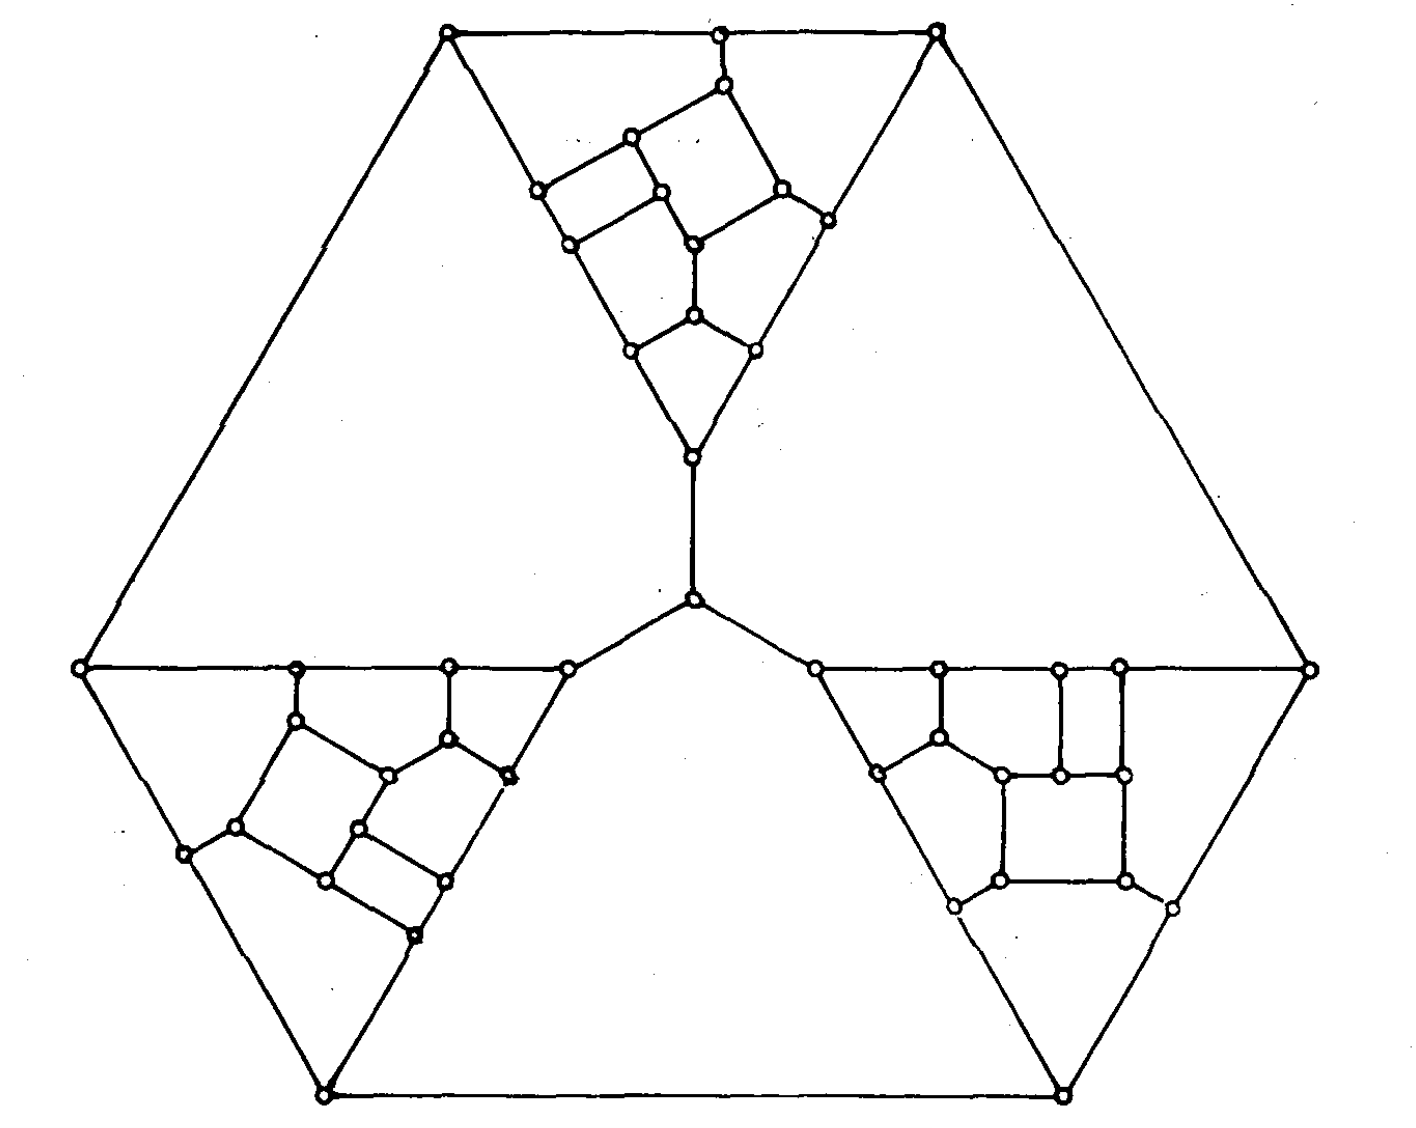
\includegraphics[width=\textwidth]{images/ceyhun1.png}

Şekil $2.6.5$ Tutte çizgesi.\\

Taite sanıtının koşullarını sağlamakla birlikte, bir Hamilton çizgesi değildir. Tutte çizgisinde $46$ düğüm vardır. Şekil $2.6.6$ da gösterilen Barnette'in önerdiği $38$ düğümlü çizge de Taite sanıtını sağlamakla birlikte Hamilton çizgesi değildir. (Okuyucu, Taite sanıtını sağlamasına karşın Hamilton çizgesi olmayan daha az düğümlü

\end{document}